%"The PDF file may contain up to 25 pages of reference material, single-sided, letter or A4 size, with text and illustrations readable by a person with correctable eyesight without magnification from a distance of 1/2 meter."
\documentclass[10pt,landscape,twocolumn,a4paper,notitlepage]{article}
\usepackage{hyperref}
\usepackage[english, activeacute]{babel}
\usepackage[utf8]{inputenc}
\usepackage{fancyhdr}
\usepackage{lastpage}
\usepackage{listings}
\usepackage{amssymb}
\usepackage[usenames,dvipsnames]{color}
\usepackage{graphicx}
\usepackage{wrapfig}
\usepackage{amsmath}
\usepackage{makeidx}

%%% Margenes
\setlength{\columnsep}{0.25in}    % default=10pt
\setlength{\columnseprule}{0.5pt}    % default=0pt (no line)

\addtolength{\textheight}{2.35in}
\addtolength{\topmargin}{-0.9in}     % ~ -0.5 del incremento anterior

\addtolength{\textwidth}{1.1in}
\addtolength{\oddsidemargin}{-0.55in} % -0.5 del incremento anterior

\setlength{\headsep}{0.08in}
\setlength{\parskip}{0in}
\setlength{\headheight}{15pt}
\setlength{\parindent}{0mm}

%%% Encabezado y pie de pagina
\pagestyle{fancy}
\fancyhead[LO]{\textbf{\title}}
\fancyhead[C]{\leftmark\ -\ \rightmark}
\fancyhead[RO]{Page \thepage\ of \pageref{LastPage}}
\renewcommand{\headrulewidth}{0.4pt}
\fancyfoot{}
\definecolor{darkblue}{rgb}{0,0,0.4}
%%% Configuracion de Listings
\lstloadlanguages{C++}
\lstnewenvironment{code}
{%\lstset{	numbers=none, frame=lines, basicstyle=\small\ttfamily, }%
	\csname lst@SetFirstLabel\endcsname}
{\csname lst@SaveFirstLabel\endcsname}
\lstset{% general command to set parameter(s)
	language=C++, basicstyle=\small\ttfamily, keywordstyle=\slshape,
	emph=[1]{tipo,usa}, emphstyle={[1]\sffamily\bfseries},
	morekeywords={tint,forn,forsn,fore},
	basewidth={0.47em,0.40em},
	columns=fixed, fontadjust, resetmargins, xrightmargin=5pt, xleftmargin=15pt,
	flexiblecolumns=false, tabsize=2, breaklines,	breakatwhitespace=false, extendedchars=true,
	numbers=left, numberstyle=\tiny, stepnumber=1, numbersep=9pt,
	frame=l, framesep=3pt,
	basicstyle=\ttfamily,
	keywordstyle=\color{darkblue}\ttfamily,
	stringstyle=\color{magenta}\ttfamily,
	commentstyle=\color{RedOrange}\ttfamily,
	morecomment=[l][\color{OliveGreen}]{\#}
}

\lstdefinestyle{C++}{
	language=C++, basicstyle=\small\ttfamily, keywordstyle=\slshape,
	emph=[1]{tipo,usa,tipo2}, emphstyle={[1]\sffamily\bfseries},
	morekeywords={tint,forn,forsn,fore},
	basewidth={0.47em,0.40em},
	columns=fixed, fontadjust, resetmargins, xrightmargin=5pt, xleftmargin=15pt,
	flexiblecolumns=false, tabsize=2, breaklines,	breakatwhitespace=false, extendedchars=true,
	numbers=left, numberstyle=\tiny, stepnumber=1, numbersep=9pt,
	frame=l, framesep=3pt,
	basicstyle=\ttfamily,
	keywordstyle=\color{darkblue}\ttfamily,
	stringstyle=\color{magenta}\ttfamily,
	commentstyle=\color{RedOrange}\ttfamily,
	morecomment=[l][\color{OliveGreen}]{\#}
}

%%% Macros
\def\nbtitle#1{\begin{Large}\begin{center}\textbf{#1}\end{center}\end{Large}}
\def\nbsection#1{\section{#1}}
\def\nbsubsection#1{\subsection{#1}}
\def\nbcoment#1{\begin{small}\textbf{#1}\end{small}}
\newcommand{\comb}[2]{\left( \begin{array}{c} #1 \\ #2 \end{array}\right)}
\def\complexity#1{\texorpdfstring{$\mathcal{O}(#1)$}{O(#1)}}
\newcommand\cppfile[2][]{
	\lstinputlisting[style=C++,linerange={#1}]{#2}
}
\begin{document}
\def\title{Universidad Autonoma de Ciudad Juarez - First to Penalty}
.\\[0.2cm]
\centering{\LARGE\textbf{First to Penalty}} \\[0.5cm]
\centering{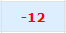
\includegraphics[width=5.5cm]{penalty.png}}
\tableofcontents\newpage

\section{Template}
\cppfile{template.cpp}
\section{Data structures}
\subsection{Simplified DSU (Stolen from GGDem)}
\cppfile{Data Structures/DSUSimp.cpp}
\subsection{Disjoint Set Union}
\cppfile{Data Structures/DSU.cpp}
\subsection{Segment tree}
\cppfile{Data Structures/SegmentTree.cpp}


\section{Graphs}


\section{Math}
\subsection{Identities}
{
$C_n = \frac{2(2n-1)}{n+1} C_{n-1}$

$C_n = \frac{1}{n+1} \binom{2n}{n}$

$C_n \sim \frac{4^n}{n^{3/2}\sqrt{\pi}}$

$\sigma(n) = O(\log(\log(n)))$ (number of divisors of $n$)

$F_{2n+1} = F_{n}^2 + F_{n+1}^2$

$F_{2n} = F_{n+1}^2 - F_{n-1}^2$

$\sum_{i=1}^n F_i = F_{n+2}-1$

$F_{n+i}F_{n+j} - F_nF_{n+i+j} = (-1)^n F_iF_j$

(Möbius Inv. Formula)
Let $g(n) = \sum_{d\mid n} f(d)$, then $f(n)=\sum{d\mid n} g(d) \mu\left(\frac{n}{d})\right)$.
}
\subsection{Binary Exponentiation and modArith}
\cppfile{Math/binpow.cpp}
\subsection{Modular Inverse (dividir mod)}
\cppfile{Math/modInverse.cpp}
\subsection{Modular Binomial Coeficient and Permutations}
\cppfile{Math/modBinCoef.cpp}
\subsection{Non-Mod Binomial Coeficient and Permutations}
\cppfile{Math/binCoef.cpp}
\subsection{Modular Catalan Numbers}
\cppfile{Math/catalan.cpp}
\subsection{Ceil Fraccionario}
\cppfile{Math/ceilfraccionario.cpp}
\subsection{Sieve Of Eratosthenes}
\cppfile{Math/sieve.cpp}
\subsection{Sieve-based Factorization}
\cppfile{Math/sievefact.cpp}
\subsection{Berlekamp Massey}
\cppfile{Math/bermass.cpp}
\subsection{Modular Berlekamp Massey}
\cppfile{Math/bermassmod.cpp}

\section{Geometry}


\section{Strings}
\subsection{Explode by token}
\cppfile{Strings/explode.cpp}
\subsection{Multiple Hashings DS}
\cppfile{Strings/multipleHashing.cpp}
\subsection{Permute chars of string}
\cppfile{Strings/permute.cpp}
\subsection{Longest common subsequence}
\cppfile{Strings/lcs.cpp}
\subsection{KMP}
\cppfile{Strings/kmp.cpp}


\section{Flow}


\section{Miscellaneous}

\subsection{Bit Manipulation}
\cppfile{Miscellaneous/bitManip.cpp}
\cppfile{Miscellaneous/moreBitManin.cpp}

\section{Testing}



\end{document}

